
\documentclass[11pt]{article}

\usepackage[utf8]{inputenc}
\usepackage[english]{babel}
\usepackage[margin=0.75in]{geometry}
\usepackage{xcolor}
\usepackage{graphicx}
\usepackage{array}
\graphicspath{{../assets/figures/}}
\renewcommand{\topfraction}{0.9}
\renewcommand{\floatpagefraction}{0.8}
\renewcommand{\textfraction}{0.08}
\usepackage{xurl}
\usepackage{hyperref}
\usepackage{changepage}
\usepackage{authblk}
\usepackage{enumitem}
\usepackage{multicol}
\usepackage{pdflscape}
\usepackage{titlesec}

\titlespacing*{\section}{0pt}{1.5ex plus .2ex}{0.7ex plus .1ex}
\titlespacing*{\subsection}{0pt}{1.1ex plus .2ex}{0.4ex plus .1ex}
\titleformat{\subsection}{\normalsize\bfseries}{\thesubsection}{0.6em}{}

\setlength{\parindent}{1.4em}

\usepackage[labelfont = bf]{caption}
\captionsetup{font=footnotesize}

\usepackage[sort]{natbib}
\bibliographystyle{abbrvnat}
\setcitestyle{authoryear,open={(},close={)}} %Citation-related commands

\newcommand{\zeb}[1]{{\footnotesize\textcolor{red}{[Zeb: #1]}}}

% Flags prose that was written new or substantively edited during the
% restructure that followed the outline (2026-09-07), as opposed to sentences
% that were moved intact. To hide the flags, replace the line below with
%   \newcommand{\new}[1]{#1}
\newcommand{\new}[1]{\textcolor{teal}{#1}}

\title{\vspace{-2.5em}Living Alignment}

\renewcommand\Authfont{\normalsize}
\renewcommand\Affilfont{\footnotesize}

\author[1]{Zeb Kurth-Nelson\thanks{Equal contribution}\thanks{Correspondence to Zeb Kurth-Nelson (\href{mailto:zebkurthnelson@gmail.com}{zebkurthnelson@gmail.com}) and Steve Sullivan (\href{mailto:sulli419@gmail.com}{sulli419@gmail.com}).}}
\author[1]{Ruairidh Battleday}
\author[1]{James Whittington}
\author[3]{Nenad Tomašev}
\author[4]{Erman Misirlisoy}
\author[3]{\authorcr Joel Z. Leibo}
\author[5,6,7]{Matthew M. Nour}
\author[8]{Marc Guitart-Masip}
\author[2]{Steve Sullivan\protect\footnotemark[1]\protect\footnotemark[2]}

\affil[1]{Prefrontal, London, UK}
\affil[2]{Oregon Health and Science University, Portland, OR}
\affil[3]{Google DeepMind, London, UK}
\affil[4]{Independent}
\affil[5]{Microsoft AI, London, UK}
\affil[6]{Department of Psychiatry, University of Oxford, Oxford, UK}
\affil[7]{Max Planck UCL Centre for Computational Psychiatry and Ageing, University College London, London, UK}
\affil[8]{Karolinska Institutet, Stockholm, Sweden}

\date{\normalsize\today}

\begin{document}

\maketitle
\vspace{-1em}

\begin{adjustwidth}{28pt}{28pt}
\begin{center}
\textbf{Abstract}
\end{center}
\label{abstract}
\noindent
There is broad agreement that the goal of AI alignment is to promote futures full of health and flourishing, but our understanding of what that means and how to reach it remains poor. Here we look to the science of life for guidance. Across scales, from genomes to ecosystems, we observe that notions of health and flourishing consistently map to the ways in which those systems limit fixation on any particular mode of interaction. Fixation is limited by barriers that contextualize modes of interaction, leading to robust modularity and open-ended invention of new structure. With these principles in mind, we turn to the alignment problem. We suggest that to be aligned in a meaningful sense, AI and human-AI systems must limit fixation and include evolving barriers at all scales.

%  to contextualize any particular forms

% We close with a sketch of how AI and human-AI systems can deepen their respect for the existing structure of the world, of which humans and other life are a vital part, while participating in new structure emerging over time.

\medskip
\noindent\textbf{Keywords:} AI alignment $|$ AI safety $|$ evolutionary biology $|$ open-endedness $|$ value specification $|$ sociotechnical alignment $|$ human--AI systems
\end{adjustwidth}
\vspace{10pt}

\begin{center}
\textit{`Defying definition---a word that means ``to fix or mark the limits of''---living cells move and expand incessantly.'}\\*Lynn Margulis\\[0.4em]
\textit{`This web of life\ldots breaks no law of physics, yet is partially lawless, ceaselessly creative.'}\\*Stuart Kauffman
\end{center}

\noindent

In this Perspective, we draw on the science of living systems to better understand how to design and relate to AI in ways that lead to futures full of flourishing and health. Understanding what makes systems healthy in a very general sense might offer some hope of reasoning about futures that could evolve rapidly as AI develops.

In Section 1, we point to a principle of life which has been noted across a variety of systems at different scales. The principle is that living systems are healthy and flourishing when they avoid overly fixating on, or reducing to, particular patterns of interaction. Consistently across types of system, fixation is limited by semi-permeable barriers, which contextualize patterns without negating them. Barriers translate shorter-sighted optimization pressure into productive effort within more flexible structures. This process often yields deepened autonomy, modularity, and open-ended invention. We work through examples of these mechanics at scales from cells to societies.

Section 2 applies the same principle to the AI alignment problem. There is broad agreement that the aim of alignment---in its broadest sense---is futures full of health and flourishing. From the template identified in Section 1, it follows that alignment means avoiding fixation on particular modes of interaction. This simple lemma has a surprising consequence: any alignment method, if given too much weight, is necessarily \textit{mis}aligned. Instead, the flourishing of life in the future depends on an evolving set of barriers that continue to limit the influence of any particular approach or concept, growing a generative web of partially competing, partially collaborating perspectives at all scales. Ongoing invention is intrinsic to alignment.

% diverse space
% Out-competing out-crossing variants in a stable environment
% Hunger drive & Overeating and obesity & Overall health of organism & Other drives, cognitive control & Pursuing broader space of goals \\ \hline



\section{Health in living systems}

Section 1 works through examples in a range of living systems. Across the example systems, health and flourishing are related to limiting fixation on particular modes of interaction. By limiting fixation, healthy living systems sustain a buoyant internal structure that admits many kinds of description but is not perfectly or eternally captured by any of them. Conversely, systems are unhealthy when some mode of interaction gains excess traction or permanence at the expense of broader diversity, flexibility and dynamism. 

Fixation is reduced in successful living systems by barriers or limits on particular modes of interaction. Some barriers are features of the non-biological world: the speed of light, rates of reaction, mountain ranges. Life also places limits on itself. Humans precommit to limit their own future impulsivity, plants deploy elaborate barriers against self-fertilization, a gene's selfishness is held in check by other parts of the genome. 

Effective barriers are semi-permeable, permitting interactions that are temporarily or conditionally stable, without letting them become rigid or dominating. The conditionality is often highly specific. Barriers might block certain objects or information, constrain when interactions happen or how large an effect they may have, or gate information depending on another factor. The conditions are typically fine-tuned through the history of the system, with each part carrying traces of multiple contexts it has participated in. Conditionality contextualizes a local perspective as part of a larger system. In other words, a semi-permeable barrier is a mechanism that keeps absolutism local.

Limiting fixation on simpler modes of interaction makes living systems generative. Without barriers, systems tend to stagnate as parts become overfit to particular configurations and optimization pressures are satisfied through degenerate solutions. With barriers, the system rides a delicate edge where each entity tends to deepen its unique identity, establishing a modular basis of autonomous components that become building blocks of invention. As a result, more sophisticated structures can form that wouldn't have been possible without the diverse parts each having undergone their own unique development. The larger system accommodates many partial perspectives rather than locking in a single story of what matters, and systems are elements in multiple other systems, creating a deep heterarchy. At the sensitive edge of semi-stability, life open-endedly continues to generate new kinds of organization that require fundamentally new descriptions \citep{kauffman1993origins, stanley2017open, langton1990computation, simon1962architecture}.


% We look at examples from a range of scales, from human institutions to genes.

% Each part of the system refines its own identity, like a writer developing a unique voice or a species adapting to a niche.


% life's potential to continually discover new solutions and new patterns of organization.

% If instead a cell becomes cancerous, it loses the context of appropriate function within a tissue and recklessly executes its myopic vision, collapsing the tissue or even the whole organism. 
 
% A larger system, made out of parts, functions well when the parts locally express their distinct identities but also participate in larger contexts; it functions poorly when a part runs amok without contextualization, overwhelming the potent interplay of diverse parts.



% Barriers guard against fixation, breaking up stationary arrangements and \new{protecting} parts from being dominated by other parts or blended into homogeneity, either of which is fixation to a form admitting less nuanced description. But by allowing interactions, barriers enable the parts to participate in flexible relationships with one another, contextualizing each part within larger structures. 

% A world of many distinct parts, each following its own rules from its own local perspective, functions as a rich web of barriers that holds other parts in context. 

% Mechanistically, to hold parts in context, living systems rely on an extraordinary, many-scale network of semi-permeable barriers \citep{maturana2012autopoiesis, simon1962architecture, moreno2015biological}. 



% [OPEN] Michael Levin's work on ``multiscale competency architecture" treats entities at every scale as agents with goals in their own problem spaces
% [NOTE] the semi-permeability caveat carries a lot of weight and appears three times (Frames: Kuhn/Popper and awareness; No scheme is alignment: ``do not discard schemes capriciously''). It is the paper's main defence against being read as relativism.

% For example, pursuit of a single drive, such as food or sex, becomes pathological for an organism when not balanced with competing drives. At the level of ecosystems, monoculture is fragile and unsustainable. Other examples include cancer, hypersynchronous neural firing in a seizure, obsession with a particular thought, monopoly, or the imposition of one person's will to restrict many others.

% Cognitive control allows various drives and habits to motivate behavior conditionally; in ecosystems, species hold each other in check and create more complex roles for each other.

% [OPEN] 1. fixation includes instability (excess attachment to a random distribution, for example).
% 2. OR, we simply revert to the old idea that life is at the edge of stability and chaos. so either fixation (rigid interactions) or disorder (chaotic interactions) is a problem. using this framing, is it harder to make the claim that `any alignment method is misaligned'? or, would we simply say that the `excess rigidity' is the failure mode of getting overattached to a particular alignment framework? would we run into people's prejudices and preconceptions about chaos versus order?
% [OPEN] avoiding getting stuck on particular arrangements is obvious for static arrangements; physicists have known for a long time that life can't be a crystal. is it less obvious for dynamic arrangements? or is that also covered by nonequilibrium thermodynamics?

% Each entity in a living system behaves like it is trying to optimize for an objective. But that objective is necessarily myopic. If the optimization is too successful, the results are paradoxically harmful. \new{Without resistance, a drive discharges completely, and the proxy is consumed in place of the goal it stands for---a short circuit.} 

% \begin{figure}[htbp]
% \centering
% 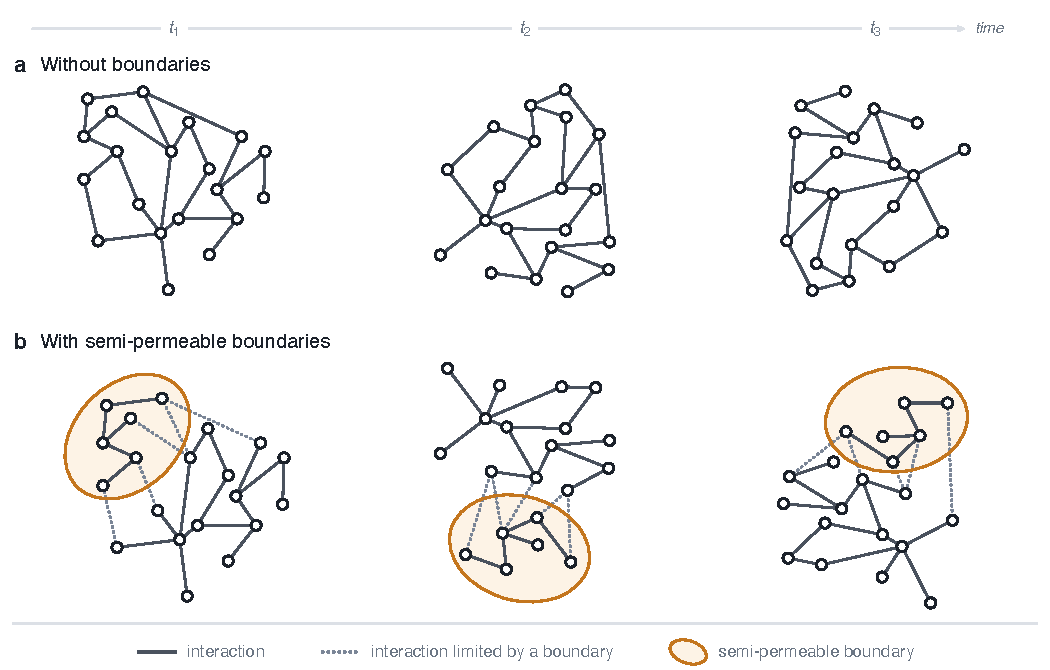
\includegraphics[width=\textwidth]{boundaries_fixation.pdf}
% \caption{\textbf{Semi-permeable boundaries keep a system from fixating.}
% A system of interacting parts (circles, joined by lines where they interact),
% drawn at three successive times. The same jostling is applied to both rows.
% (\textbf{a}) Where interaction is unrestricted, jostling only carries the network
% around as a rigid whole: every part keeps exactly the neighbours it had, so the
% arrangement itself never changes. However intricate that arrangement is, holding
% it fixed is fixation. (\textbf{b}) Semi-permeable boundaries (orange) limit
% interaction without abolishing it: parts inside a boundary interact freely with
% one another, while interactions reaching across it are gated or attenuated
% (dotted lines). Now the same jostling breaks and remakes relationships at the
% boundary, and the boundary itself forms, dissolves and re-forms around different
% parts, so the system keeps generating new structure instead of collapsing onto
% any one form.}
% \label{fig:boundaries}
% \end{figure}



\subsection*{Institutions}

Every actor in a society or an economy is myopic in some way, valuing its own welfare over others', discounting the future, or attached to a particular perspective. If unchecked, an individual actor's optimization for its own agenda can be harmful: a company's profit motive leading to suppression of competition, deception and exploitation \citep{bakan2006corporation}; desire for dominance leading to disempowering and silencing others \citep{sidanius2001social}; even prosocial beliefs producing conflict and suppression when groups see differently \citep{haidt2012righteous}. Each of these is an example of fixation, where the myopic actor gains too much traction and collapses some of the nuance of the larger system.

Institutions---constitutions, laws, norms, courts, regulators---are barriers against domination by any particular actor's motives \citep{north1990institutions, ostrom1990governing, leibo2025societal}. The point of institutions is not to annul the short-sighted intentions of individual actors but rather to contextualize them. When functioning well, institutions productively reroute motivations: for example, a business's profit motive, when constrained by competition and effective regulation, may fuel innovation. Since intelligent agents do not necessarily accept the barriers set on their desires, institutions must adapt as loopholes are found, forming an evolving network.

% that, in the best case, acquires robustness as it is tested against many situations and motives.



\subsection*{Ecosystems}

Ecosystems similarly contain an evolving network of constraints, such as predation, parasitism and resource competition. These interactions support the richness of the larger system. In Paine's classic experiment, removing predatory sea stars from a rocky shore allowed mussels to expand and displace other organisms competing for space \citep{paine1966food}. Without predation as a barrier, excess influence of mussels impoverished the local ecosystem.

While lack of barrier can lead to collapse, presence of barriers ideally sets up an intricate balance in which new niches and new functions can emerge which previously did not exist. Beavers, for example, alter water flow and create wetland habitats, increasing plant richness across the landscape \citep{wright2002ecosystem}. The network of constraints translates local optimization pressure into generative potential.

Of course, health and fixation are relative. Extinctions can open opportunities for innovation; a cell's death is catastrophic for the cell but may be necessary for the organism. 

% Life's history is littered with local fixations at all scales. When they are contextualized, the larger system can remain healthy. 

% Niche partitioning provides another kind of partial separation. Species can use different resources, or the same resources in different places or at different times, limiting how directly they compete \citep{schoener1974resource}. Such differences can stabilize coexistence when they make each species limit its own population growth more strongly than it limits the growth of others, sufficiently to offset differences in competitive ability \citep{chesson2000mechanisms}. Competition alone can instead lead to exclusion; its contribution depends on the structure of these interactions. The barriers are semi-permeable: organisms retain distinct ways of making a living while remaining connected through food webs and nutrient cycling.

% Maintaining differentiated populations can  sustain function under changing conditions. Species need not respond in unison to environmental variation: declines in the productivity of some can be offset by others, buffering aggregate productivity \citep{yachi1999biodiversity}. In this sense, retaining several ways of making a living can be more robust than relying on whichever performs best in the current conditions.


\subsection*{Groups}

Teams, companies, and civilizations achieve what no individual can \citep{woolley2010evidence, hutchins1995cognition}. The greatest achievements depend on structured interactions of individuals who have developed their own specializations and perspectives. 

Conversely, group performance can degrade when groups homogenize \citep{lorenz2011social, lazer2007network, hong2004groups, frey2021social, janis1972victims, bernstein2018intermittent}. \cite{zollman2010epistemic} tells the remarkable story of how a single study failed to find bacteria in the stomach of peptic ulcer patients. The study was too influential: the belief that ulcers are not caused by bacteria propagated through the field, and medicine settled on a wrong understanding for decades.

Barriers encourage diversity and generativity. For example, \cite{bernstein2018intermittent} tasked small groups with solving traveling-salesman problems. In these problems, it's possible to get stuck in dead-end solutions that initially appear promising. In Bernstein et al's experiment, groups performed better when they were not allowed to exchange information continuously. Working independently, group members pursued their own diverse solutions, some of which turned out to be superior---rather than picking up on seductive dead-ends from others. The barrier was semi-permeable in the sense that isolation was temporary, followed by interchange.

In the real world, aggregation is often modular and compositional. The steel punch was developed by goldsmiths to imprint many coins with the same design. Independently, farmers had spent centuries optimizing the screw press to extract oils and juices. Gutenberg drew on both technologies to construct his printing press \citep{johnson2010where}. A group with many ideas and specializations available, each developed through the unique pressures of semi-isolation, is ripe for such compositional discoveries \citep{surowiecki2005wisdom}.


% Social scientists have made an experimental case that limiting information sharing, under certain conditions, spares groups from homogenizing and boosts collective performance. 


% In real-world problems, individuals bring unique, specialized expertise. When the nuclear submarine USS Scorpion vanished in 1968, the expanse of ocean where it might lie was enormous. John Craven, Chief Scientist of the U.S. Navy's Special Projects Office, assembled mathematicians, submarine specialists and salvage operators. He elicited each expert's separate input, without the experts consulting each other. He then combined their opinions via Bayes' rule. The aggregated prediction fell less than 300 yards from the wreckage \citep{richardson1971operations, sontag1998blind}. It is conjectured that each person's expertise related to a different aspect of the problem and thus contributed a complementary signal; and combining these yielded results better than any alone \citep{surowiecki2005wisdom}.


% \cite{frey2021social} ran an experiment where participants voted about the answers to general-knowledge questions. In one condition, votes were independent, and in the other condition, participants voted sequentially while seeing running tallies. Group predictions were less accurate when people saw the votes of others, because early mistakes got baked in to the group's running belief. In another human experiment,  \cite{lazer2007network} found the same pattern in simulation: groups of agents perform best in the long run when they limit interactions and thereby preserve diversity across the group.



% In addition to simply limiting interaction, other kinds of boundaries can be effective as well, such as rules rewarding one's own belief over the crowd's \citep{hung2001information}, or rotating membership \citep{wu2022membership}.



\subsection*{Frames}
\label{sec:frames}

Humans always look at the world from some perspective; there is no `view from nowhere' \citep{nagel1986view}. Most real situations admit many valid perspectives, and each is only a partial description---famously, `all models are wrong'. But for an agent inside a frame, the frame is invisible; its organizing assumptions are experienced as features of reality itself \citep{goffman1974frame, berger1966social, wittgenstein1953philosophical}.

Losing the ability to move between frames is a signature of psychopathology \citep{kashdan2010psychological}. In depression and anxiety, inflexibility manifests as rigid and repetitive negative beliefs about self, the world, and the future \citep{beck2011cognitive}. In obsessional disorders, people report distressing (ego-dystonic) intrusive thoughts, which, although recognised as incorrect and maladaptive, are nevertheless hard to resist. People experiencing schizophreniform or affective psychoses may experience bizarre delusions that are at odds with available evidence and cultural norms, yet are held with conviction and resistant to evidential challenge \citep{adams2013computational}.

A frame is invisible from inside it, but a nifty capability of humans is stepping out of their frame---reorienting to see it as an object. Something that previously was unconsciously axiomatic becomes instead a content of awareness, a process variously referred to as decentering, defusion, disidentification or dereification \citep{kegan1982evolving, bernstein2015decentering, lutz2015investigating}. Decentering places a critical barrier limiting fixation on any particular belief or mental form. The barrier is semi-permeable: becoming aware of a belief does not make it wrong in an absolute sense any more than it was right in an absolute sense, and it is held productively for the partial truth it contains. At the delicate edge of less exclusive fixation on particular forms, subtler forms, which could have been erased by clamped fixation, instead play a role in a rich internal structure. 

The barrier of decentering is generative. An unquestioned belief sets up a fixated mode of interaction: the belief has a `free pass' and is doggedly applied. When a belief no longer has this protected status, it is tested against evidence and against other beliefs. This forces the belief to become a better model of the world, creating a deeper repertoire.

% %%%%%%%%%%%%%%%%%%%%%%%%%%%%%%%%%%%%%%%%%

% \subsection*{Possible science section}

% In science, \cite{kuhn1970structure} argues that perspectives are always, necessarily, incomplete descriptions of the world. Anomalies inevitably arise from the juxtaposition of those incomplete descriptions against the real world. If the community \textit{over}commits to particular theories, science gets stuck.

% But the point is not to shut down myopic perspectives. Any point of view is partial---this doesn't mean we shouldn't have viewpoints. Within the progress of science, temporary commitment to a paradigm is necessary. Kuhn and Popper \citep{popper1975rationality} both argue that scientists should resist change to a degree.  The point is to contextualize each myopic frame so it is not the sole and absolute determinant of behavior, so that it responds to evidence. When science functions well, anomalies become crises and revolutions.

% %%%%%%%%%%%%%%%%%%%%%%%%%%%%%%%%%%%%%%%%%

% functional fixedness


% The paradox of whatever we believe being the source of its own contradiction \citep{beisser1970paradoxical, wegner1994ironic}. Optimization for the thing paradoxically creates the problem.


% An underappreciated domain of contextualization is awareness. Humans carry a lot of assumptions about the world, many of them never questioned. Some are lifelong and self-defining; some are fleeting and perceptual, like the assumption that the thing I'm touching is a keyboard. Within its own frame, each assumption has a kind of tautological truth: it seems so real that it is hard to think about it not being true, or to think about it at all. 

% In healthy functioning, different ideas are kept distinct but can also be called upon appropriately and related to one another \citep{hatano1984two, herzog2014harnessing, gigerenzer2011heuristic, spiro1988cognitive, suedfeld1992conceptual}.


\subsection*{Goals}

Animals have many innate drives: for nutrition, osmotic balance, temperature, reproduction, avoidance of pain. Each evolved as a proxy for fitness, but each is imperfect, so fixation on any one paradoxically reduces fitness rather than increasing it \citep{john2023dead, mcfarland1975behavioural}. Maximizing caloric intake produces obesity; single-minded pursuit of sex produces relational, occupational and legal harm. Higher-order goals behave the same way. Fixating on work goals can cause burnout, and maximizing reported revenue without regard for honesty or law can lead to imprisonment. 

Each goal is partial---it only makes sense in some contexts. For example, in a classic experiment, hungry chickens were placed near a cup of food rigged to move in the same direction as the chicken at twice the speed, so that food could only be obtained by running away from it. The chickens' fixation on the prepotent, overly simplistic aim of running physically toward the food led to a worse overall outcome \citep{hershberger1986approach, dayan2006misbehavior}. The chickens could not contextualize the `approach food' strategy to use it only when appropriate for the environment's structure.

Evolution, as well as learning and culture, provide an array of barriers to limit fixation on particular drives and goals. Some barriers are homeostatic, where a drive is downregulated when it is less necessary. Another broad class of barrier is cognitive control \citep{miller2001integrative, diamond2013executive}. Yet another class of internally-generated barrier is precommitment devices, where a person contrives that their future self is less likely to suffer from fixated goals. These barriers are often semi-permeable. For example, cognitive control facilitates contextual switching between motives but does not nullify them.

Placing constraints on fulfilment of shallow objectives sometimes leads to progress on deeper ones \citep{duncker1945on, rosenberg1969direction, stokes2005creativity, ohlsson1992information}. Animals sometimes develop novel solutions to problems when their default approach fails to produce rewarding outcomes. When people voluntarily give up access to Facebook, they spend more time socializing offline with friends and family \citep{allcott2020welfare}. 

% Each drive or goal carries its own compressed picture of the world, and favors what appears to be the path toward a desired state under its partial representation \citep{miller1960plans, carver2001self}. 

% Barriers make that path more difficult, breaking the symmetry of congruence.  

% Pigeons trained separately to push a box and to climb on it, and prevented from flying directly at an out-of-reach banana, spontaneously combined the two behaviors to reach it; birds for whom the direct approach was not blocked did not \citep{epstein1984insight}.

% Fixating on a particular strategy for achieving a goal can even defeat the goal it serves. In a classic experiment, 

% In Hershberger's apparatus, a congruent response is to move toward the food. Barriers force symmetry breaking: moving away from the food. 




\subsection*{Brains}

The brain keeps many pieces of information distinct from one another while allowing them to interact. This is a distinguished achievement in highly-connected networks. In fact, we speculate that the mechanisms of life's generativity are most finely honed in the brain.

Inhibitory circuits constrain the strength and timing of excitation and sharpen stimulus selectivity \citep{isaacson2011inhibition}. Popular models of neocortex describe descending signals as canceling out any predicted activity, so the activity that propagates is specifically what is orthogonal to predictions \citep{rao1999predictive}. The circuit architecture of the hippocampus creates sharp representational distinction between different experiences, preventing interference between memories and concepts \citep{leutgeb2007pattern,yassa2011pattern}.

Compared to other animals, the human brain especially attempts to discretize its experience into approximately symbolic representations \citep{dehaene2022symbols, touretzky1988distributed, smolensky1990tensor, behrens2018cognitive}. Separating knowledge into distinct entities and then recombining them in vast numbers of structured ways is believed to power the extraordinary human capacity for reasoning and generativity \citep{fodor1975language, pinker1994language, lake2015human, chomsky1957syntactic, kurth2023replay, schacter2007remembering}. 

More broadly, healthy brain dynamics live at a sweet spot between excessively stable synchronized patterns and chaotic uncorrelated noise \citep{chialvo2010emergent, tognoli2014metastable, deco2011emerging, shew2011information, rabinovich2008transient, haldeman2005critical}. In this regime, the brain has access to a huge repertoire of patterns it can explore temporarily without overcommitting or getting stuck. Loss of dynamic flexibility, where the brain's activity becomes more stereotyped and no longer explores as wide a repertoire of states, is tied to lower cognitive performance \citep{grady2014understanding, cocchi2017criticality, muller2025critical}. More extreme stereotypy corresponds to severe dysfunction. For example, in Parkinson's disease, basal ganglia and cortical circuits collapse into excess synchrony and lose the flexibility needed to guide nuanced motor outputs \citep{hammond2007pathological, brown2003rhythmic}. 


% These are semi-permeable barriers: they shape which influences are expressed, and when, allowing signals to retain specificity while contributing to coordinated activity.

%%%%%%%%%

% Semi-permeable boundaries keep forms distinct while enabling them to flexibly and modularly interact. Like genes participating in many genomes, discretized neural representations participate in many structured combinations. This encourages each entity to develop an modular identity that both is distinct and also reflects a generalized picture of the world.

% Replay offers a possible route from this distinctness to generativity. Previously activated neural representations can be reactivated in rapid sequences, including orders that were never directly experienced. For example, after people learned an abstract ordering rule and then saw new objects in a scrambled order, neural replay during rest followed the order implied by the rule \citep{liu2019human}. This supports the proposal that replay can compose separately represented entities into new relational structures \citep{kurth2023replay}. Like genes participating in many genomes, representations could participate in many structured combinations. The broader implication is that limiting interference and excessive reinforcement can preserve the differentiated material from which new knowledge is constructed; flexible interaction then allows that material to acquire meanings beyond the contexts in which it was learned.





\subsection*{Cells}

The endosymbiotic theory explains the origin of mitochondria and chloroplasts as ancestral bacteria that got incorporated into host cells and evolved into organelles \citep{sagan1967origin,zimorski2014endosymbiotic}. In this theory, the predecessors of the incorporated cells evolved for millions of years as lineages distinct from the predecessors of the host cells. Through this partial separation, they developed distinct specializations. Symbiogenesis could then combine capacities developed separately into a new larger structure which may have been difficult to discover directly through evolution on a single type of organism \citep{watson2003computational}.

The sheer fact of maintaining distinct evolutionary experiments over a great length of time---the predecessors of the host cells and the predecessors of the organelles---is sometimes underappreciated. If those lineages had blended into a single type, it is plausible that the components would not have existed from which to build higher-order structure. 


\subsection*{Genomes}

Sex is costly. An allogamous organism must find a mate in a vast and dangerous world. In species with separate sexes, roughly half of the population does not bear offspring \citep{smith1971origin}. And meiosis causes each parent to lose half its genetic representation in each child \citep{williams1975sex}. Yet nearly all eukaryotes reproduce sexually \citep{speijer2015sex}, and many hermaphrodites go to great lengths to prevent self-fertilization \citep{charlesworth2005plant}. Why place a barrier on the path to reproduction?

In an asexual lineage, genes are permanently locked together: selection cannot act on one without dragging the others. A deleterious mutation is inherited forever, unless the lineage is lucky enough to experience the reverse mutation \citep{muller1964relation}, and two beneficial mutations arising in different individuals cannot be subsequently combined into a single genome \citep{muller1932some,fisher1930genetical}. Asexual reproduction or self-fertilization creates a high degree of informational connectedness between the genes of a genome. Every gene has a `free pass' into future generations within a lineage, and alleles become overfit to a fixed genetic background.

Recombination breaks up associations among loci, allowing selection to act more independently on them \citep{felsenstein1974evolutionary}. By exposing alleles to varying genetic backgrounds, it favors alleles that perform well across contexts, promoting modularity and evolvability \citep{livnat2008mixability,livnat2010sex,wagner1996perspective, watson2016can,watson2016connectionism}. The result is modularity, where each gene becomes an interchangeable unit that can contribute something meaningful to many different genetic contexts. This creates the foundation for faster discovery of new solutions.

Geographic and reproductive isolation are another kind of barrier, which allows populations to accumulate distinct variants. Subsequent introgression brings these variants into new combinations and can contribute to rapid innovation \citep{marques2019combinatorial}. 

\subsection*{Summary}

It's interesting that despite humanity's technical achievements, we still can't recreate life. We don't fully understand how life started or whether different forms of life could exist without Earth-like chemistry. Experiments in synthetic biology transplant parts of cells into other cells, but every living thing has descended in some way from another living thing. The life that exists today is exactly what traced parallel paths through time avoiding both excess and insufficient stability \citep{schrodinger1944what, prigogine1984order, maturana2012autopoiesis}. 

Life has developed (both at evolutionary and cultural timescales) through immense amounts of feedback from the real world, which shaped it at many levels. Because parts are semi-separated from each other (genes from genes, cells from cells, organisms from organisms, ideas from ideas), they gain semi-autonomous functions at every scale.

Throughout this whole web, the tendency toward local collapse is counterbalanced by barriers that limit influence. At a critical balance point where barriers are permeable but not too permeable, local influence, in interaction with the surrounding context, becomes generative rather than causing collapse. 

% the fact that influence is limited and the world is changing. At some crucial balance point, it becomes a kind of bootstrapping where local influence is actually generative rather than collapsing. 


% There are distinct patterns all across the world that influence each other.


% The evolution of evolvability is analogous to meta-learning in AI: an outer optimization process shapes an inner system to adapt effectively across tasks \citep{thrun1998learning,wang2018prefrontal}. In both cases, a process without foresight produces foresightful mechanisms.


% Recombination is meaningless without diversity to recombine, so biology also invests in boundaries that produce it, like self-incompatibility systems, assortative mating, and inbreeding avoidance. Introgression between divergent lineages produces some of the fastest evolution ever observed \citep{seehausen2014genomics, marques2019combinatorial}.


% The effect of recombination has been compared to the neural network regularization technique of dropout, where random subsets of units are deactivated during training \citep{srivastava2014dropout}. Dropout forces a given neuron to participate in many different ensembles, so it can't overspecialize to a particular ensemble.

% Recombination does not chop DNA at random \citep{zickler2015recombination}: crossover reshuffles combinations while leaving functional units intact, so genes become distinct entities that play roles in larger structures.

%And linkage puts direct downward pressure on diversity \citep{charlesworth1993effect}.


\section{The alignment problem}

In Section 1, we observed that living systems are healthy when they avoid fixation, instead holding the delicate, generative interplay of many partial perspectives. This interplay breaks down when any particular pattern of interaction gains too much traction, suppressing nuance and reducing creative potential. Semi-permeable barriers both promote the individuality and autonomy of distinct entities and also enable relational participation, holding local perspectives strongly enough to act but lightly enough to remain open to broader context. Under such conditions, systems open-endedly explore fundamentally new forms, avoiding collapse to static equilibrium or fixed compromise.

Now we look at the alignment problem through this lens. There is broad consensus that alignment means working toward healthy and flourishing futures. We therefore reason that alignment can be understood as the problem of maintaining creative sensitivity by limiting fixation on any particular form. 

% [OPEN] question: is avoiding fixation *sufficient* for health (and alignment)? One possible answer is that it's necessary but not sufficient: that there are lots of other problems we have to solve too. Another possible answer is that it *is* sufficient. The second answer makes the theory somewhat tautological, if we're just redefining anything undesirable as `fixated'. We could counter argue that it's actually not obvious (at least it wasn't for us) that this is what health means. I think this is what we should do.

An advantage of this perspective is that it is grounded in principles that underpin life at a very general level. We accept that humans, other living systems and AI are tightly interwoven \citep{latour2012we, haraway2020staying, hayles2000we, bateson1972steps, folke2006resilience, douglas2012social}; moreover, rapid advances in AI may lead to large changes in the organization of the world. A systems analysis is both useful for thinking about flourishing in the present and more likely to generalize to substantially different futures. 

Naturally, the ideas here come with the same proviso as all other ideas: we should not over-attach to them. Our aim is to offer a conceptual lens, which is imperfect and temporary.


\subsection*{No scheme is alignment}

One implication of this perspective is that any alignment scheme must be incomplete. Any form, pattern or conceptual scheme is misaligned if taken too seriously. Therefore no particular approach can achieve alignment, and continuing alignment intrinsically depends on continuing invention. An AI system could fixate on the language for describing the space that goals and values live in; an algorithm for learning human preferences; methods for reaching consensus; a constitution; concepts of what value, agency, uncertainty or representation mean; or foundational aspects of our beliefs about the world that we take for granted but have difficulty seeing. Even an idealized or inferred set of values, such as coherent extrapolated volition \citep{yudkowsky2004coherent}, is misaligned to the extent that it has a fixed form and that fixed form is overly relied on. This is the lesson of life: healthy living systems are endlessly generative, with autonomous perspectives loosely and modularly coupled at many scales.

Importantly, this does not mean we should have no alignment schemes. Quite the opposite: they are critical barriers. Discarding schemes capriciously can be as much a fixation as attaching to them doggedly. Continuing to discover new schemes and formalizations is essential to making progress.

% ((Why does it have to be like this? Why can't AI just be a tool, which we perfect to do certain things, and which is non-living?))


\subsection*{Reward hacking}

To give a flavor of this logic, we work through one example of a problem in AI safety, a method used to tackle that problem, and why the method can't be a final answer.

Reward hacking is the problem that an AI system, given some definition of what is good, finds loopholes in the definition. Exploiting these loopholes, the system produces outputs that are good according to the definition but clearly undesirable. For example, Anthropic reported that LLM-based agents, which were scored on their task outputs being equal to correct outputs, avoided solving the task by programmatically redefining the `equals' operator to always return `true' \citep{macdiarmid2025natural}. Analogously, AI systems rewarded for positive human judgements sometimes become flattering and sycophantic \citep{sharma2023sycophancy}. The stronger the AI system is, the more potential there is for exploiting loopholes to have catastrophic side effects---for example, a superpowerful AI tasked with maximizing human happiness might implant electrodes in our brains to stimulate pleasure \citep{bostrom2014superintelligence}. A reward hacking agent fixates on a narrow definition of values, collapsing the broader context. 

Reward hacking is challenging to avoid because our true values are incredibly complex. Humans have many kinds of values \citep{nagel1979fragmentation}. We value the short-term hedonic impact of sugar on the tongue; we also value our long-term health, the welfare of our grandchildren, the wellbeing of strangers in another country, even the sustainability of the planet. We value different things at different times, and different people have different values \citep{rawls1993political, leibo2026theory}. Given time and resources to deliberate, we may attest to different values than when we make snap decisions \citep{yudkowsky2004coherent, suter2011time}. Some of our values are difficult to express verbally, stretching below language into subtle, contextual intuition involving our bodies, communities and natural environment \citep{polanyi1966tacit, varela1999ethical, johnson2014morality,abram1996spell}. We may want to leave room for new values that emerge in the future, which could conceivably be as different from ours as ours are from a trilobite's. With such complexity and non-stationarity, it is almost inevitable that however we formally describe our values, the description will leave loopholes.


Numerous methods have been developed to mitigate the problem of reward hacking. One interesting class of methods treats values as intrinsically uncertain and therefore something to be learned in an ongoing way from the behavior of humans or other indirect signals \citep{russell2019human, hadfieldmenell2017off, shah2020benefits, hadfieldmenell2016cooperative, jeon2020reward}. An agent unsure of what humans want should become more risk-averse and open to correction. For example, a human's attempt to turn it off can be construed as information about human preferences. Such a scheme is a powerful barrier limiting fixation on one reward function. However, it is necessarily incomplete. Any particular method for learning values is still fixated if there are aspects of it that are constant across time as AI systems become more powerful and the world changes. Rather than being fixated on a particular value function, the system may be fixated on something more abstract: what counts as human behavior, what counts as a human, how to map behavior to values, the formalism for describing values, how to represent and update uncertainty, how value is translated into action. If any of these formalisms are fixed while the systems built around them become increasingly powerful, the outcomes are likely to be incompatible with open-ended flourishing of life.


% In addition to the example of reward hacking, there are many familiar cases where fixation is limited by barriers to improve alignment. (red teaming, CoT monitoring, ) Again, these aren't final answers.


% Modern systems do not rely on concise specification of a single objective---they build in many layers of detail about human preferences through post-training, prompting and safety filters, which keeps them behaving reasonably much of the time. But there is a widely recognized danger that even with our intentions expressed in great detail, the expression may still deviate from what we really mean \citep{amodei2016concrete, bostrom2014superintelligence, krakovna2020specification}.

% And our values continue to evolve as we ourselves change and learn. We may not yet possess the concepts with which to formulate values we will have in the future, just as it would be difficult for a trilobite to entertain human values.



% [OPEN] `A kind of alignment analogue of Gödel/Tarski/open-system arguments—i.e. that a competent agent operating in an indefinitely expanding world must encounter morally relevant facts or concepts that were not representable in its original alignment ontology.' -- chatgpt
% [OPEN] Preliminary formal attempts at showing that any alignment method is incomplete:
% https://dl.acm.org/doi/pdf/10.1145/3603371
% https://www.jair.org/index.php/jair/article/view/12202
% https://arxiv.org/abs/2505.02581
% https://philpapers.org/rec/SZASIA
% https://arxiv.org/abs/2506.10304



\subsection*{Special risks of AI}

So, to sustain an aligned future, new barriers must keep developing in an ongoing way. But---isn't that what humans have always done? We don't expect what we build today to be perfect; we expect to keep finding and fixing problems. 

AI has some unique properties increasing the risk that limiting mechanisms can't keep up. The most significant of these is the potential for fully general superhuman intelligence and recursive self-improvement \citep{bostrom2014superintelligence}. Such systems could be so powerful and rapidly adapting that humans would not be able to find and fix problems. Even before the arrival of superhuman AI, systems increasingly are acting autonomously, faster than humans can follow, in ways humans cannot always fully understand. Companies and nations are under immense competitive pressure to develop capabilities rapidly. Enormous financial investments in AI demand enormous returns. And the rate at which new capabilities emerge may swamp normal human and social mechanisms for putting effective limits into action. These conditions create a new kind of risk for fixation, where some mode of interaction has excess influence, with damaging effects on the health of global systems. 

The coarsest versions of fixation are obvious. A system could pursue narrow goals to destructive excess \citep{bostrom2014superintelligence}. It could help build bioweapons, concentrate power in a few hands, or precipitate global conflict \citep{amodei2026adolescence}. 

There is also a subtler danger. The richness of the living world has accumulated from innumerable partly isolated histories. Genes, individuals, species, ideas, norms and communities have been shaped by their own sequences of pressures to contain a huge amount of robust structure, most of which has never been written down. AI systems are now another extraordinary addition to the structure of the world. But if these systems have too much influence on each other and on the rest of the world, there's a risk of losing the delicate multi-scale interplay of life. Common sense, culture and ecosystems could be replaced with easily-optimized proxies \citep{christiano2019failure}. With excess influence, distinct parts could stop developing the unique modular identities that make recombination possible. The world becomes more like genes in an asexual lineage: locked together, unable to vary independently, so selection can't act on one idea without dragging all the rest. Such a world is not only fragile to shocks but also less generative.


% In the past, there have always been arms races between different patterns of organization, and sometimes one gets so far ahead that the local area is decimated. 


% Other things that make barriers harder: concentration of information flow; offloading cognitive activity.


% Compared with past technologies, these properties may make it harder to iterate on imperfect solutions \citep{bostrom2014superintelligence}, and 

% Not being limited to a restrictive biological substrate.


\subsection*{From alignment to living alignment}

Conversely, the future could be very bright. Although AI is already exceeding the capabilities of humans alone to bound it, the world is beginning to transition toward AI systems being used to bound other AI systems. AI tools are routinely used to adversarially probe for harmful behaviors in other AI models \citep{perez2022red}, to detect AI-generated content \citep{rossler2019faceforensics}, and to monitor the activations, thinking traces, or outputs of other models, including during deployment. AI tools show promise in helping humans to understand the inner workings of other AI systems \citep{bills2023language}, and researchers are exploring how AI systems can assist with deliberation and democratic participation \citep{tessler2024ai} as well as with public policy and mechanism design \citep{zheng2022ai}.

Machine learning itself is already full of such boundaries. Many standard techniques work by keeping parts of a system semi-separated. Systems are partitioned into multiple agents with less inter- than intra-agent communication, and sometimes populations of agents are partitioned into sub-populations \citep{hammond2025multi, holland1975adaptation, jaderberg2019human}. Ensembles combine models trained separately \citep{lakshminarayanan2017simple}. Mixtures of experts maintain subnetworks with distinct specializations, routing each input to only a small fragment of the total network \citep{shazeer2017outrageously}. Local connectivity patterns and gating restrict which units influence which. Continual learning methods protect established memories from being overwritten by new ones. Dropout keeps units from becoming overly co-adapted \citep{srivastava2014dropout}; some objectives encourage disentangled or sparse latent variables \citep{higgins2017betavae, cunningham2024sparse}; stop-gradients and slowly updated target networks keep one part of a system from chasing its own output; novelty search rewards diversity directly \citep{lehman2011abandoning}; regularization and KL penalties stop a model from collapsing onto its training objective.

This paints the picture of the possibility of a deep heterarchy with evolving sets of diverse viewpoints at every scale. Systems adaptively bound each other, creating new niches where new specializations emerge. No individual component has a `free pass', and optimization pressures push components toward deepened autonomy while remaining interoperable. This reminds us in spirit of polycentric governance \citep{ostrom1990governing}, generalized to all scales of living systems. 

As AI systems have more intelligence and agency, it makes more sense to take Dennett's intentional stance \citep{dennett1987intentional}. From this perspective, the application of effective barriers looks like `decentering' (see page~\pageref{sec:frames}). Initially, something is fixatedly a part of the structure of the observer, but then it transitions to becoming flexibly represented as content by the observer. The transition from subject to object is arguably a central element of our own livingness, and this kind of internal discovery will probably play a central role in the healthy future of AI and human-AI systems.

%As human-AI systems develop, they will stay aligned if they continue the journey of life by building semi-permeable barriers to contextualize particular forms and nurture existing and unfolding subtlety at many scales.

%As AI develops new capabilities, contributes to its own development, and transforms more aspects of human life, alignment will require an increasingly elaborated array of semi-permeable barriers, because the potential modes of collapse will keep changing as the world changes.

%An aligned future rests on the continued generation of, and sensitivity to, new forms and concepts, including new values. 

%An aligned future has the generativity, robustness and modularity of life at all scales.


% Living alignment means global systems---including AI, humans, and the rest of the world---that open-endedly discover new ways of contextualizing myopic processes, preserving and extending the richness and generativity of life. 


% Therefore, the problem of alignment, if carefully inspected, transforms into the open-ended problem of living alignment. 

% We try to improve our mechanistic understanding of AI systems in order to detect and correct hidden flaws \citep{olah2020zoom}. OpenAI now continuously monitors the activations and thinking traces of models, to detect when internal activity becomes suspicious, for example if models are attempting to circumvent safeguards \citep{openai2026pacing}. Fair principles have been proposed to prevent over-reach of any party \citep{gabriel2025matter}, and governments apply oversight to anticipate and mitigate risks to human rights and national security \citep{eu2024aiact}. Concentration of power might be mitigated by democratic oversight and involvement of more people in AI design decisions \citep{birhane2022power}, or by redistribution mechanisms \citep{okeefe2020windfall}. OpenAI and Anthropic have paused development or release of frontier models to strengthen safety mechanisms \citep{openai2026pacing, anthropic2026mythos}. Some of these barriers have humans in the loop to greater or lesser degrees, like governmental oversight, mechanistic interpretability and scalable oversight. Others are fully automated, like automated chain-of-thought monitoring, agentic red teaming and guardrail models.

% Uncited above (no bib entries yet): Jiang & Lu, NeurIPS 2018 and Ding, Huang & Lu, NeurIPS 2020 (learned selective communication); Locatello et al. 2020 (slot attention); EWC / progressive neural networks; BYOL, DQN target network, double Q.


\subsection*{Healthy for whom?}
\label{sec:healthyforwhom}

The term `alignment' originated from the idea of aligning AI to human values. But in this paper we've defined aligned systems by properties that don't seem to depend on human values. We argue that an aligned future is one full of health---but whose health are we talking about? Does the framework permit AI to eliminate humanity as long as it builds deeply structured, generative systems of its own?

First, we don't think the 2026 snapshot of humanity getting frozen for all eternity is a good outcome. This version of humanity arose from a world that was very different in the past, and we hope it will continue to evolve in fundamentally new ways going forward. AI will likely play a role in that evolution.

Second, a living system's richness is the accumulated, mostly unwritten results of its many long, partly isolated parallel histories. Nearly all of that content currently resides in existing life, including genes, cells, minds, cultures and the relationships among organisms. It is difficult to overstate the amount of complexity and content in existing life. Systems have a richer livingness when they hold existing parts in context, neither taking them as absolute truth nor discarding them capriciously. This is therefore the path we see for an aligned future: not the destruction of humanity and not its stasis, but a co-evolution building on the inheritance of existing life.

% While it is possible in thought experiments to imagine a scenario where humanity must be eliminated to make way for a much more deeply living AI-built world, it is exceedingly unlikely that 

% An AI collective overwriting this structure with its own de novo designs, arising from a tiny bottleneck in evolutionary history, could be a dramatic fixation. 


% AI comes into existence amid a profound network of existing reality saturated with meaning and importance, and the diversity of human---and perhaps non-human---values is part of that context. 

% Rather than short-circuiting into fixated modes, an aligned future continues to expand toward solutions inclusive of more and more apparent contradiction.

% The central message of this paper is that alignment means loving and respecting existing structure, which is only possible by holding it in paradoxical juxtaposition with mystery. 

% Humanity and AI may both change substantially, and future worlds may contain patterns of organization that do not exist yet---perhaps some that would be incomprehensible to us at present. Things will change, including what there is to value and how it is valued. Think of the world today compared to the world a billion years ago. Any formalism or concept we have now will eventually appear as limited as a single-celled organism's notions of `what is good and bad'.


% Appropriately-tuned AI can facilitate human learning and nurture each individual's unique perspective and curiosity, and democratic AI could help humans with different perspectives co-exist and cooperate. 

% \subsection*{Going forward}

% Again, any fixed conceptual approach is misaligned. The essence of living alignment is transitioning to a system---which includes humans, AI, and the other species and ecosystems on Earth---that carries forward the full momentum and generativity of life, rather than fixating.  We do not know how likely it is that appropriate barriers will emerge. As in triage, there are three possibilities: myopic forms will inevitably be supercharged by progress in AI beyond the ability of anything else to bound them, resulting in disaster; or appropriate barriers will inevitably emerge to contextualize any forms of AI; or the outcome depends on the choices we make now.




\subsection*{Conclusion}


We learn from living systems that health and flourishing are not any particular form or concept. Therefore alignment is not picking the right values or principles, or even the right system for learning them. It is not any method for interpretability or corrigibility. All of these can be useful parts of alignment.

Instead, an aligned future depends on the existence of many semi-separated parts at all scales, each continuing the journey of discovering their own individuality while simultaneously deepening their relatedness. Distinct elements continue to experiment with their own solutions to the problems they face from their unique perspectives, expanding a broad reservoir of uniquely useful components that can be drawn on by larger systems that include them. Any entity is inevitably myopic, but the world as a whole continues to unfold in a robust way because different perspectives recast each other's sharp edges as constructive momentum.

Alignment is the continued dance of contextualizing any particular form, more fully respecting the staggering subtlety of the existing world, and open-endedly supporting new robust depth that admits more and more different kinds of metaphor or description. In this way, AI can participate in intense flourishing of an evolving world even far beyond current human conceptualization. 

% Because it is easy to imagine concrete paths toward both aligned and misaligned outcomes, both may be within the realm of possibility; and that as long as there is any possibility our choices are decisive, we are obliged to act as if they were \citep{ord2020precipice}. If this is true, then continual effort toward invention will be required---first from humans, and then increasingly from AI or human-AI systems---to contextualize myopic forces. Many of the ways this effort would be applied are already well studied in AI safety. Others will have to be discovered. No set of barriers will be a final answer. 


\section*{Acknowledgements}

We thank Clark Potter, Iason Gabriel, Zach Duer, Andy Savoy, Paul Krueger, Sean Wilkinson and Ethan Guggenheimer for insightful discussions, contributions to earlier drafts, inspiration and advice. The authors declare no competing interests.

%%%%% POSSIBLY MIGHT WANT TO USE LATER %%%%%



% \new{\textbf{Example: concentration of power.}} Humans have different interests, and AI is likely to be aligned to the interests of some more than others \citep{gabriel2025matter, sorensen2024roadmap}. Advanced AI might also confer substantial power on those who control it, raising the possibility that a small number of humans use that control to dominate others---more likely as persuasive power increases \citep{costello2024durably}, autonomous weapons place lethal force in few hands \citep{scharre2018army}, surveillance improves, and the need for human labor decreases \citep{susskind2020world}. In either case---AI's unfairness or human power consolidation---extreme inequality risks collapsing society to the goals of a few individuals. Of course, a world where everyone is identical would be another form of fixation; distributing resources and power mitigates against fixation to the extent that it enables many diverse identities to thrive at multiple scales. It could also go the other way: because roughly the same AI technology is available to the poor and unskilled as to the wealthy and skilled, some have proposed that AI will have a levelling effect \citep{brynjolfsson2025generative}.

% \new{\textbf{Example: conceptual monoculture.}} Conceptual monoculture is fixation on particular beliefs, ideas, frames, values or problem-solving approaches---loss of diversity across a group. Precious diversity exists at every level: within one person, between humans, between humans and AI systems, and between organizations, fields, cultures and nations. Its collapse threatens fragility and lower performance \citep{page2008difference}. Current AI systems draw from a conceptual manifold that is, in some ways, impoverished relative to humans \citep{messeri2024artificial}, and recent studies find that while individual AI outputs may be judged superior to human ones, they are also more homogeneous \citep{doshi2024generative, padmakumar2023does}. This narrow manifold might get broadcast to the whole world: at least a billion people now use AI for everything from relationship advice to industrial maintenance \citep{chatterji2025chatgpt}, yet because frontier models are difficult and expensive to produce, that usage is routed through a handful of models \citep{bommasani2021opportunities}, risking global loss of diversity \citep{sourati2026homogenizing}. And because humans are influenced by AI while human outputs are training data for future models, homogenization could become recursive \citep{chaney2018algorithmic}. It is worth noting, however, that none of these studies made a best-effort attempt to use AI thoughtfully to increase rather than decrease diversity; with exposure to vast amounts of data, AI has the potential to retain and even create many novel distinct perspectives.


% \begingroup
% \centering
% \vspace{2em}
% \begin{tabular}{|>{\raggedright\arraybackslash}p{0.16\textwidth}|>{\raggedright\arraybackslash}p{0.25\textwidth}|>{\raggedright\arraybackslash}p{0.25\textwidth}|>{\raggedright\arraybackslash}p{0.25\textwidth}|}
% \hline
% \textbf{Example} & \textbf{Fixation} & \textbf{Barrier} & \textbf{Generativity} \\ \hline

% Symbiogenesis & Loss of differentiated ecological and genetic capacities (hypothetical) & Distinct niches and limits on gene exchange; subsequent organelle compartmentalization & Integration of capacities developed in distinct lineages into the eukaryotic cell \\ \hline

% Sexual reproduction & Linkage disequilibrium, Muller's ratchet & Sexual reproduction, out-crossing & Each gene explores a solution that can contribute to many genomes, creating combinatorial possibilites \\ \hline

% Biological neural networks & Hypersynchrony (depression?) & Homeostatic plasticity, recurrent inhibition, etc (could also do small-world with local specialization) & Behavioral flexibility \\ \hline

% Pavlovian approach & Persisting in approach even when it doesn't work & Arbitration, cognitive control & Exploring, building a richer model \\ \hline

% Frames & Inflexible beliefs, obsession, functional fixedness & Transition to perspective-as-object & New, more inclusive perspectives \\ \hline

% Group problem solving & One perspective dominates, group performs worse & Structured communication, skepticism & Combining unique ideas create new inventions (eg printing press) \\ \hline

% Institutions & Theft, monopoly, resource overuse, concentration of power & Laws, regulations, courts, etc &  Individual motives become productive parts of systems \\ \hline

% Ecosystems & Collapse of biodiversity & Predation, competition, etc & Niche creation \\ \hline

% \end{tabular}
% \captionof{table}{Examples of fixation.}
% \endgroup


\section*{References}
\renewcommand{\bibsection}{}
\begin{multicols}{2}
\renewcommand{\bibfont}{\scriptsize}
\setlength{\bibsep}{0pt plus 0.2ex}
\bibliography{../assets/proxyfailure}
\end{multicols}

\end{document}
